\section{Gesture Recognition}

\begin{frame}{How to Control Devices}{}
A look at the following subset of our system:
\begin{itemize}
    \item Gesture Recognition
    \item Point Detection
    \item User Orientation
    \item User Position
\end{itemize}
\end{frame}

\begin{frame}{Gesture Recognition}{}
Two types:
\begin{itemize}
    \item Image based
    \item Motion based
\end{itemize}
\end{frame}

\begin{frame}{Gesture Recognition}{}
\centering
\begin{figure}
    \subfloat{
        \frame{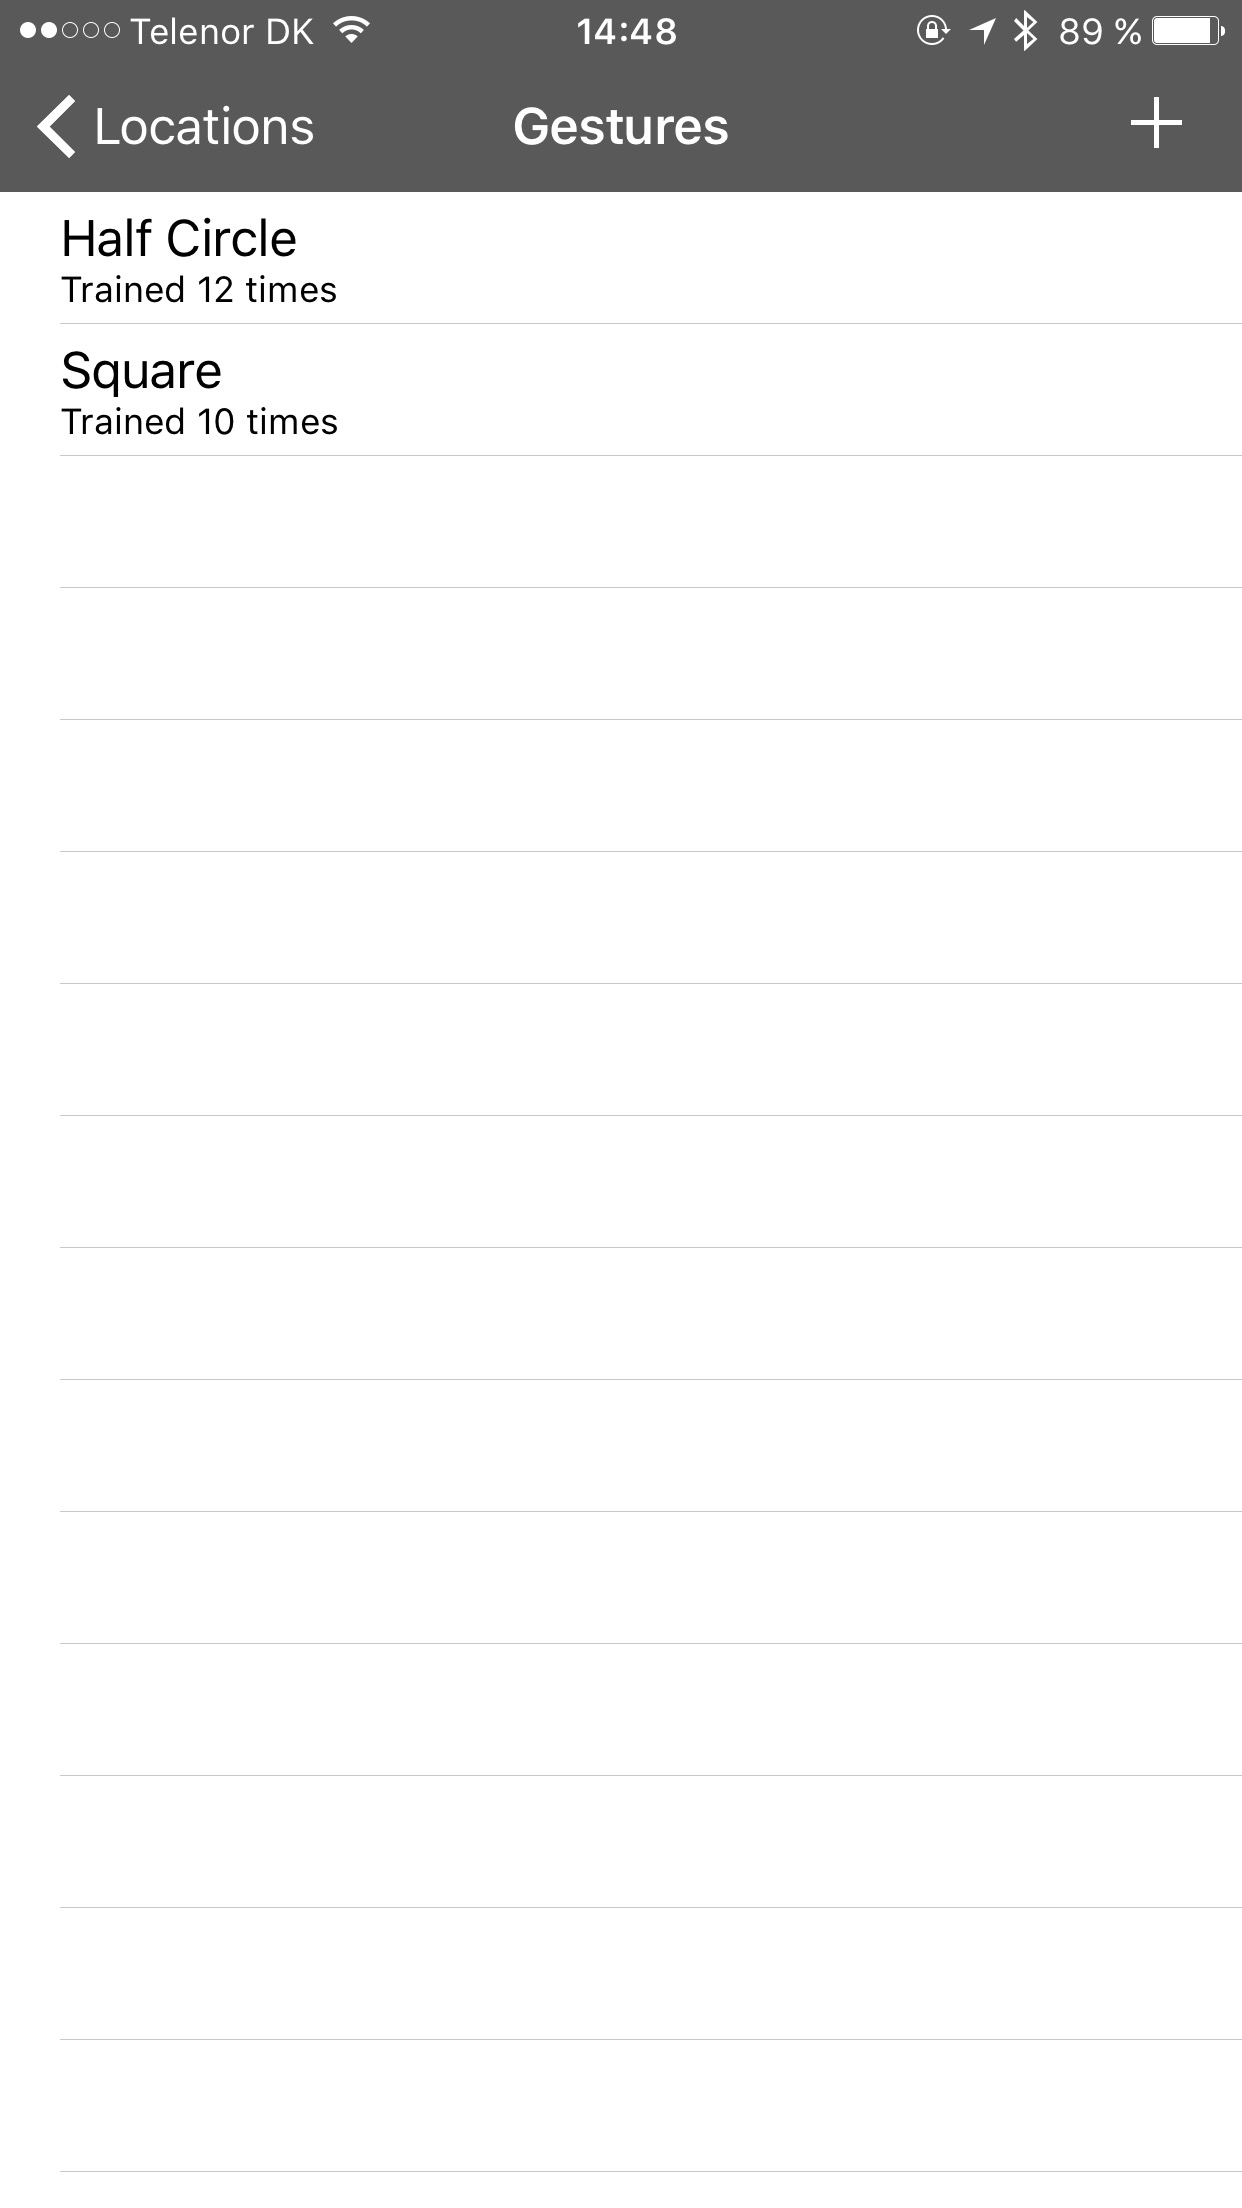
\includegraphics[width=0.3\textwidth]{../images/prototype-3-all-gestures}}
    }
    \subfloat{
        \frame{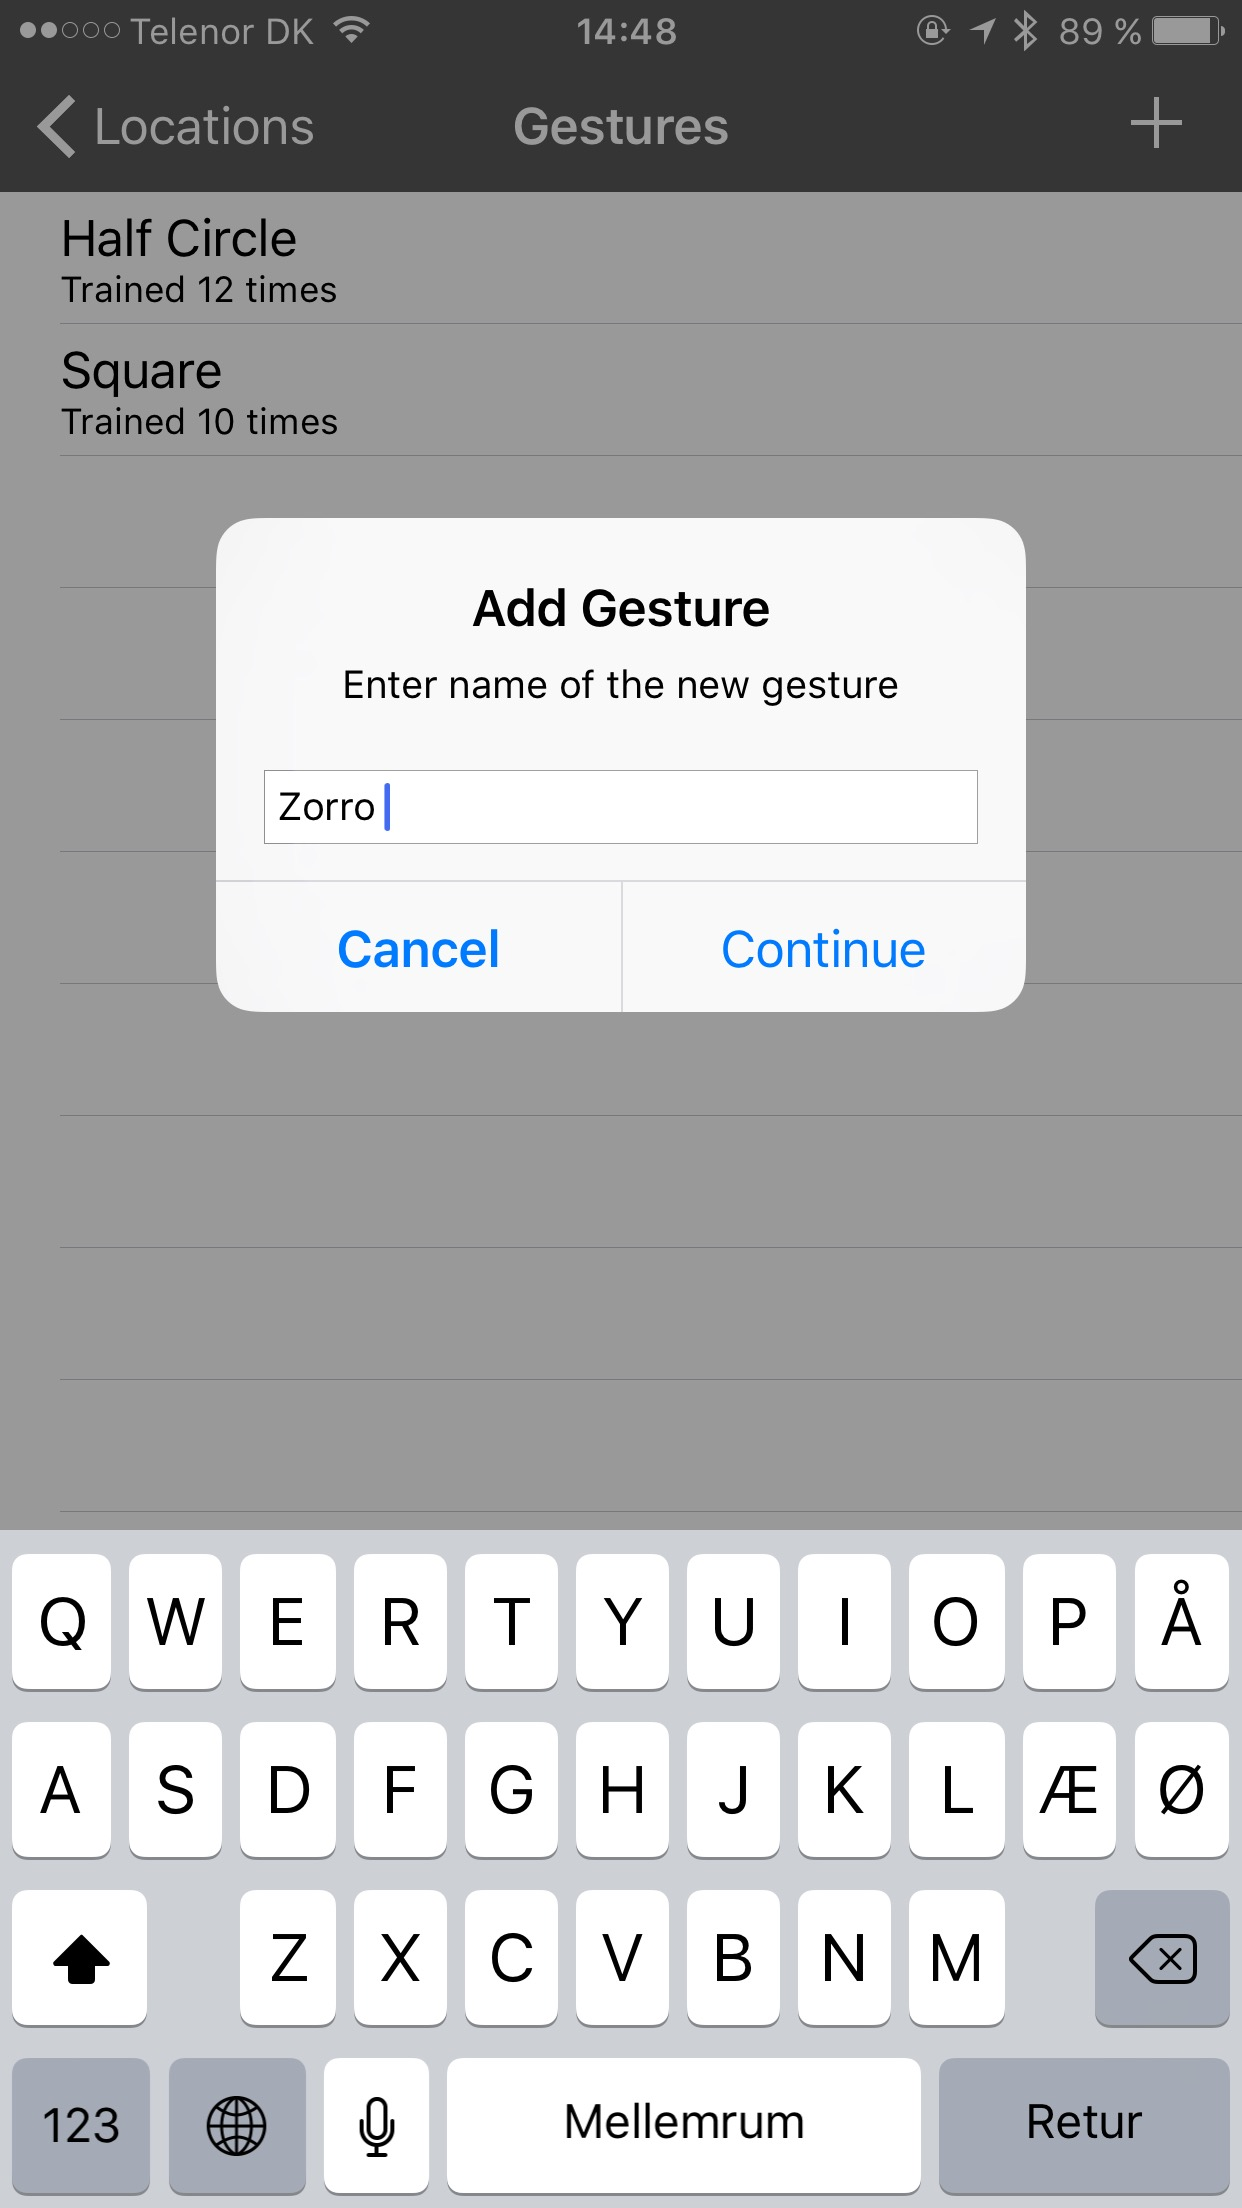
\includegraphics[width=0.3\textwidth]{../images/prototype-3-new-gesture}}
    }
    \subfloat{
        \frame{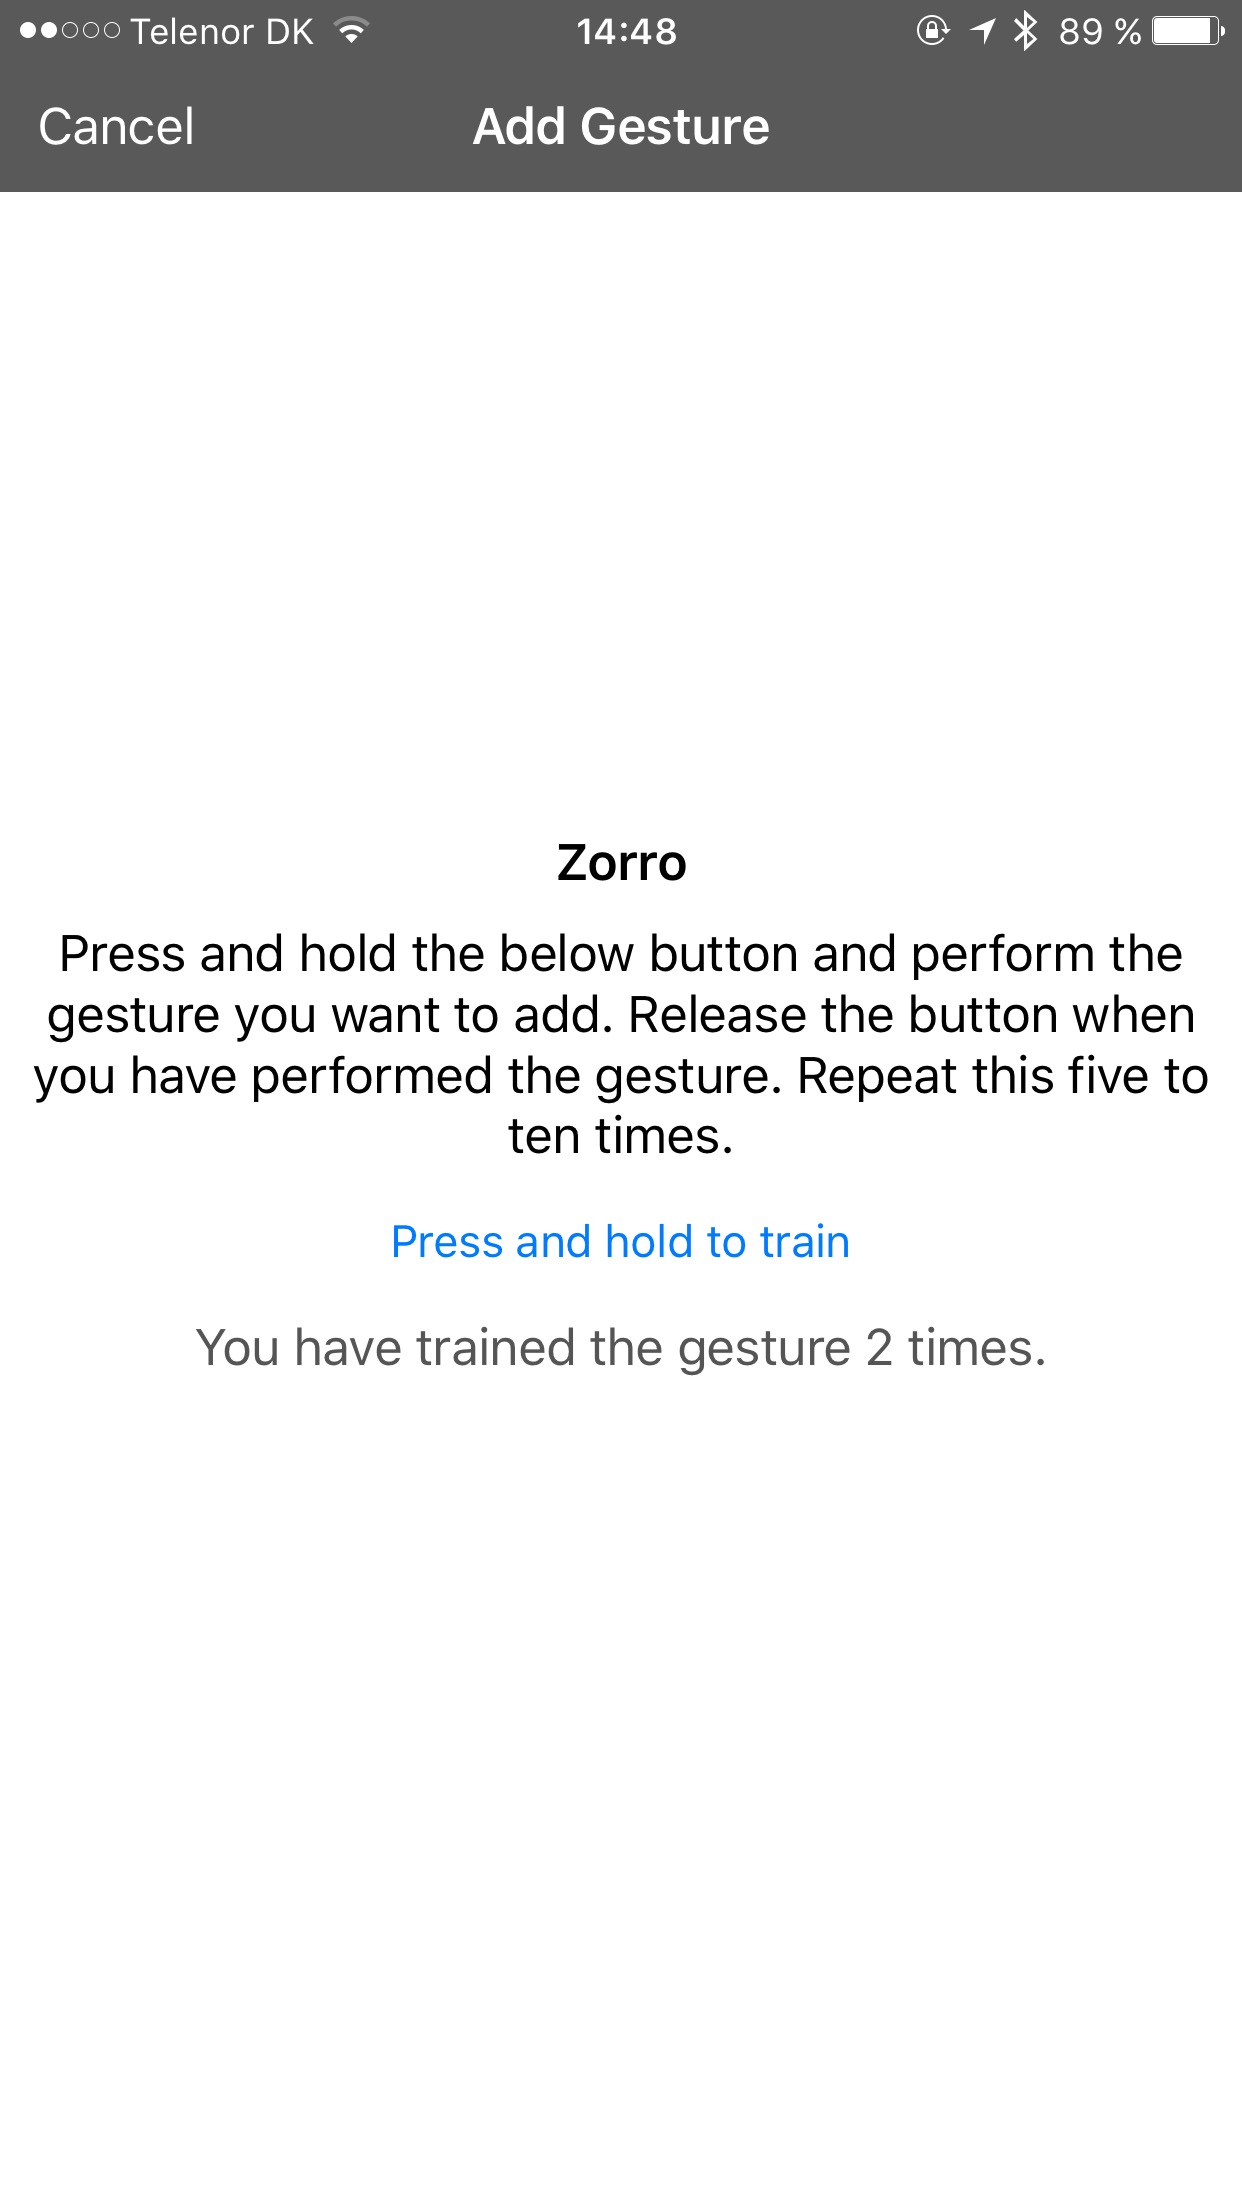
\includegraphics[width=0.3\textwidth]{../images/prototype-3-train-gesture}}
    }
\label{fig:prototype3-gesture-screenshots}
\end{figure}
\end{frame}

\begin{frame}{Gesture Recognition}{Point Detection}
\begin{figure}
    \frame{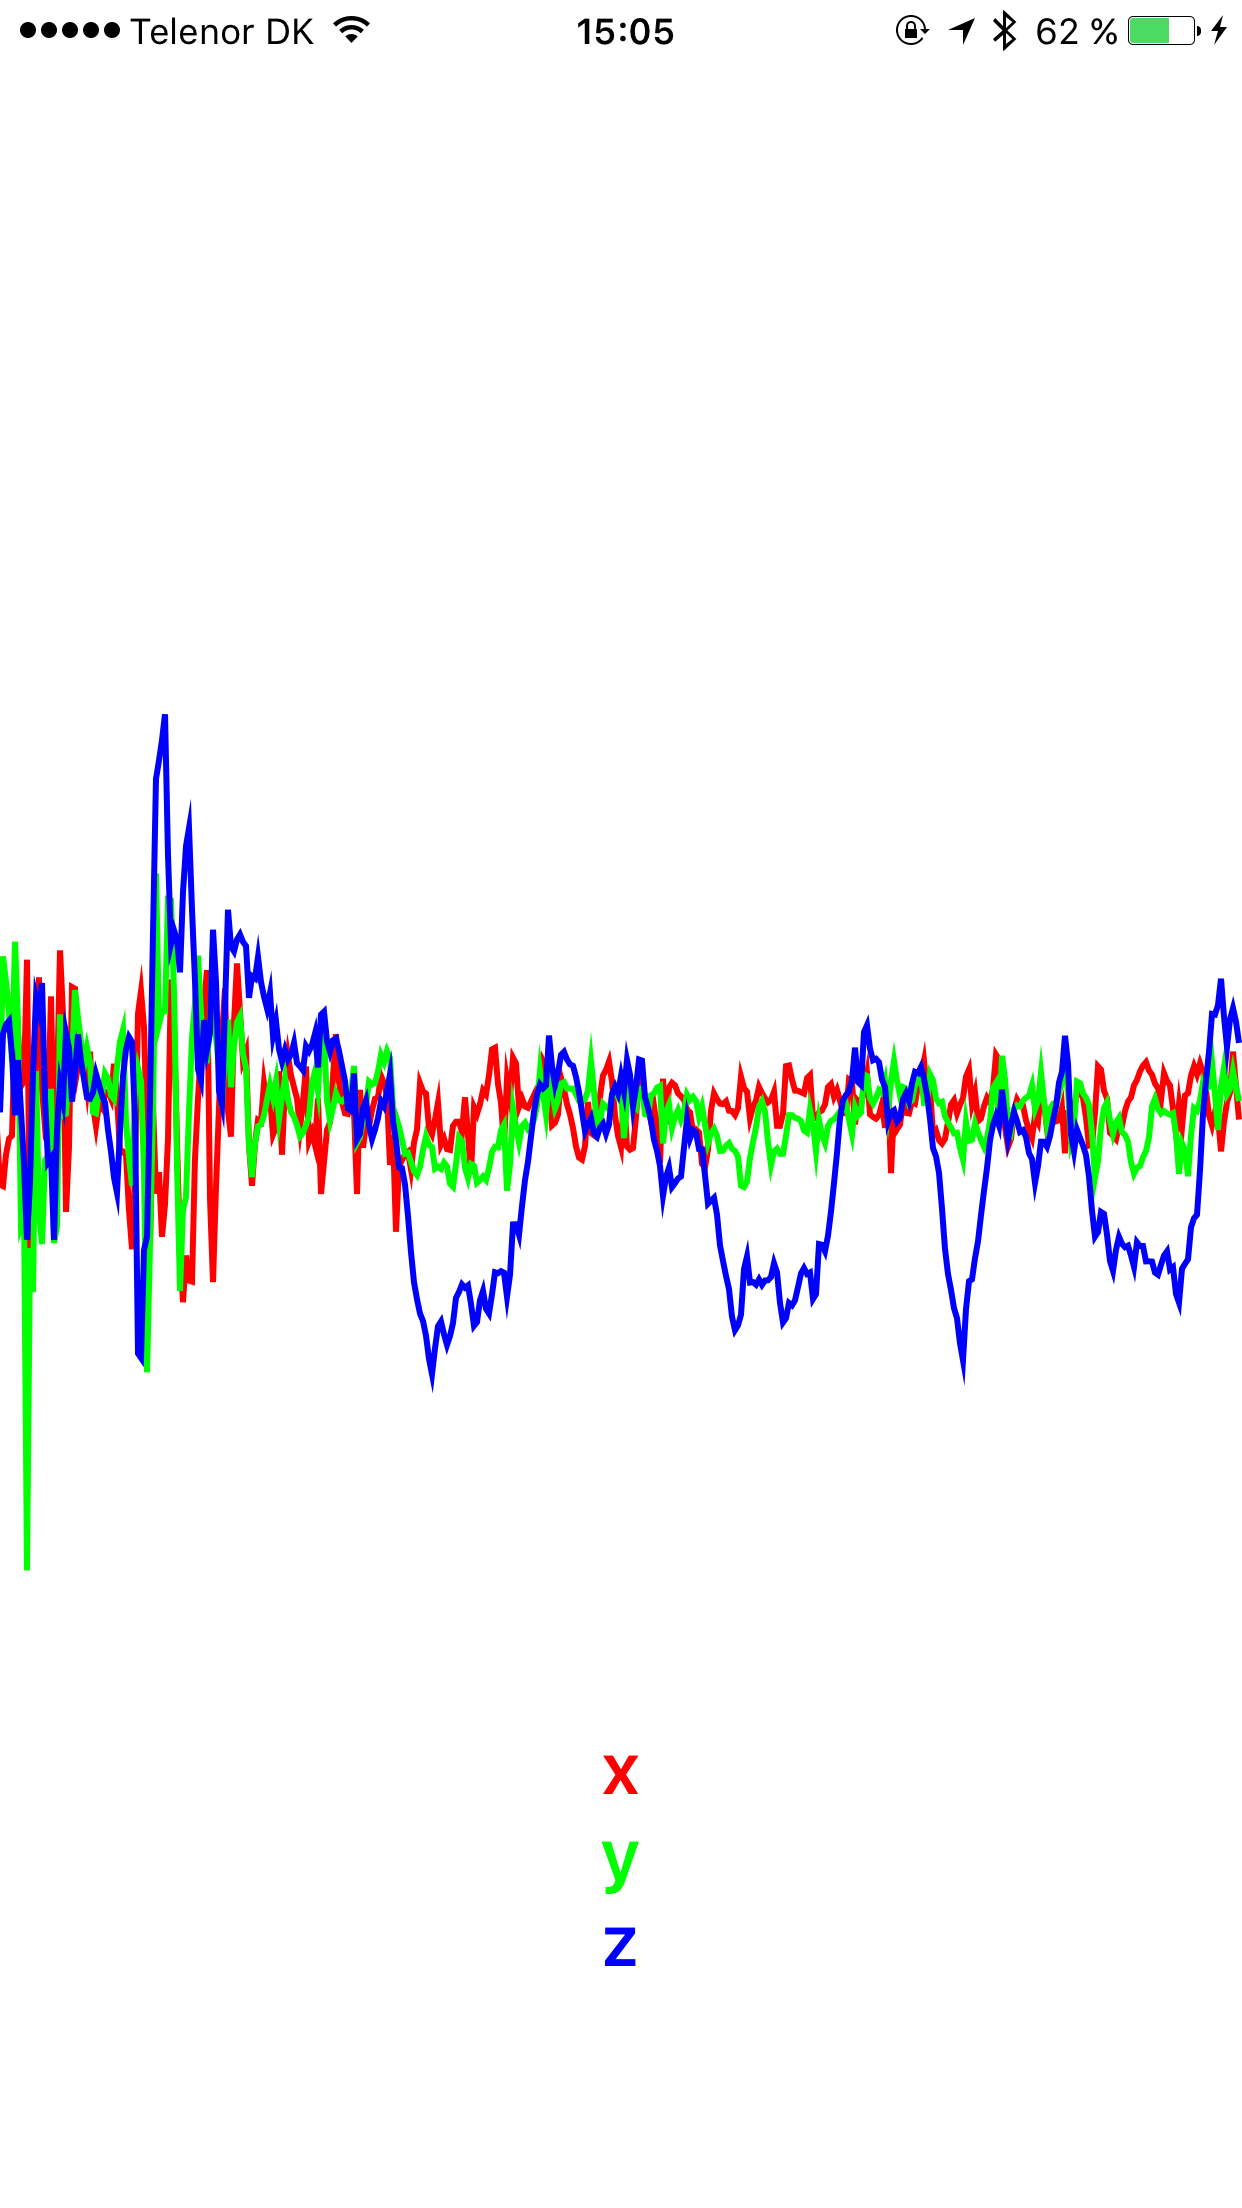
\includegraphics[width=0.3\textwidth]{../images/pointer-walk}}
\end{figure}
\end{frame}

\begin{frame}{Gesture Recognition}{Point Detection}
\centering
\begin{figure}
    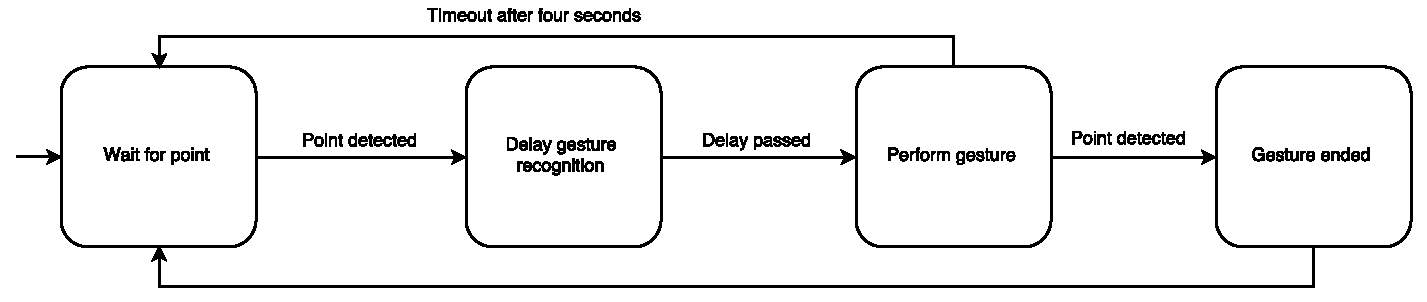
\includegraphics[width=\textwidth]{../images/point-to-gesture-state-diagram}
\label{fig:point-to-gesture-state-diagram}
\end{figure}
\end{frame}